% Springer Nature journal manuscript; project draft, not a submitted article.
\documentclass[pdflatex,sn-mathphys-num]{sn-jnl}
% Project reading copy: compact margins. Set false for publisher defaults.
\newif\ifcompactdraft
\compactdrafttrue
\ifcompactdraft
  \geometry{reset,a4paper,left=25mm,right=25mm,top=26mm,bottom=25mm,
    headheight=5.5pt,headsep=5.6mm,footskip=10mm,bindingoffset=0mm}
\fi
\usepackage{graphicx}
\usepackage{amsmath,amssymb}
\usepackage{booktabs}
\raggedbottom

\begin{document}

\title[EEG sleep staging and reference profiling]{EEG Sleep Stage Classification with Targeted N1/N2 Spectral Refinement and Reference-Based Recording Profiles}
\author[1]{\fnm{Om} \sur{Ahuja}}
\author[1]{\fnm{Rikin} \sur{Parekh}}
\affil[1]{\orgdiv{Information and Communication Technology},
\orgname{Pandit Deendayal Energy University}, \orgaddress{\country{India}}}

\abstract{This project investigates five-class EEG sleep staging, targeted correction of N1/N2 predictions, and descriptive recording profiles. A retained Fast SCFormer-U checkpoint processes four EEG channels in 30-second epochs. Nine spectral features feed a balanced logistic-regression refiner fitted exclusively on training epochs with both true and baseline-predicted labels in N1/N2. At inference, routing depends only on the baseline prediction. A 24-recording subset of the Haaglanden Medisch Centrum database contains 15,216 training, 3,619 validation, and 3,109 test epochs. On the same four test recordings, refinement increases accuracy from 55.45\% to 59.34\% and macro F1 from 57.42\% to 59.51\%. Of 238 changed predictions, 154 become correct and 33 become incorrect, yielding 121 net additional correct epochs. The pipeline also computes sleep architecture and spectral summaries and compares them with a reference derived from 16 training recordings. Sleep Studio presents hypnograms, raw and refined evaluations, uncertainty, and report exports. These results establish a reproducible project baseline; the small test cohort, incomplete recording coverage, and absence of external clinical validation limit generalization. Reference deviations describe this clinical training cohort and are not diagnoses or validated severity estimates.}

\keywords{Sleep staging, EEG, spectral features, N1/N2 refinement, reference profiles, reproducibility}
\maketitle

\section{Introduction}\label{sec:introduction}
An epoch classifier provides a stage label, but reviewing a recording also requires understanding where predictions disagree and how those errors affect the estimated sleep pattern. We address these needs in one workflow: four-channel EEG is labeled in 30-second intervals, a spectral model revisits selected N1/N2 decisions, and the resulting sequence is summarized for inspection. The five output classes are Wake, N1, N2, N3, and REM.

The retained classifier exhibits substantial N2-to-N1 confusion: 506 of 1,283 true N2 test epochs are initially assigned N1. The implemented refinement asks whether complementary spectral features can improve this distinction while retaining the existing checkpoint. The project contributions are a prediction-routed N1/N2 refiner, a training-reference profiling workflow, and a desktop application connecting inference to review and reporting. This manuscript documents the implemented experiment and its retained evidence rather than claiming a new evaluation of the underlying classifier.

\section{Related work}\label{sec:related}
Earlier staging systems differ in how they combine signal representation with information from neighboring epochs. DeepSleepNet learns features from a single EEG channel using convolutional layers and incorporates bidirectional recurrent processing~\cite{supratak2017}. SeqSleepNet introduces a hierarchy in which one level represents individual epochs and another processes an epoch sequence~\cite{phan2019}. This distinction matters for the present implementation: its attention and recurrent layers operate inside each 30-second input. A learned model spanning consecutive epochs remains future work.

The HMC database and its associated inter-database study provide a clinical data source and context for evaluating transfer across datasets~\cite{hmc2022,alvarez2021}. PhysioNet provides the hosting platform~\cite{pollard2026}. Published scores from other cohorts, modalities, and protocols are not directly comparable with this project's small subset. Accordingly, the results below compare only the retained classifier and its targeted refiner on identical stored test inputs.

\section{Dataset and experimental protocol}\label{sec:data}
The HMC Sleep Staging Database version 1.1 describes 151 clinical polysomnography recordings, with four EEG derivations sampled originally at 256~Hz~\cite{hmc2022}. The current experiment uses 24 stored preprocessed recordings. Table~\ref{tab:split} gives the retained partition sizes. Partition membership is fixed in the saved split metadata. Recording IDs are disjoint across training, validation, and test sets. A repeated-night person mapping is not supplied; recording disjointness alone does not independently establish person-level independence.

\begin{table}[htbp]
\caption{Stored inputs for experiment HMC-N1N2-20261007.}\label{tab:split}
\centering
\begin{tabular}{lrr}
\toprule
Partition & Recordings & Epochs \\
\midrule
Training & 16 & 15,216 \\
Validation & 4 & 3,619 \\
Test & 4 & 3,109 \\
\midrule
Total & 24 & 21,944 \\
\bottomrule
\end{tabular}
\end{table}

The held-out recording IDs are SN001, SN004, SN009, and SN022. Stored SN001 contains only 190 epochs, equivalent to 95 minutes, so its outputs describe a segment. Stored NPZ sequences preserve epoch order, but the present experiment has not independently verified their whole-night coverage, continuity, or alignment with lights-out markers.

The original checkpoint was selected by validation evidential accuracy, with checkpoint epoch 9 retained from a 10-epoch history. The current experiment loads that checkpoint and fits the refiner using the training partition only. Test labels are used for evaluation, never for inference routing. The draft reports descriptive point estimates; it does not claim statistical significance or external validation.

\section{Methods}\label{sec:methods}
\subsection{Preprocessing and retained classifier}
The channel order is F4-M1, C4-M1, O2-M1, and C3-M2. The documented preprocessing selects channels, applies a 50~Hz notch at the original sampling rate, applies a 0.3--35~Hz bandpass, and resamples to 100~Hz. Each 30-second epoch therefore contains a $4\times3000$ array. Per-channel, per-epoch normalization is
\begin{equation}
 \widetilde{x}_{c,t}=\frac{x_{c,t}-\mu_c}{\sigma_c+10^{-6}}.
\end{equation}
Exact checkpoint reproduction includes the notebook's second normalization of stored epochs at inference. Spectral features use the stored EEG before this second normalization. The retained configuration does not support a claim of amplitude-based artifact rejection.

Fast SCFormer-U combines Conv1D layers with 64 and 128 filters, four-head self-attention, a BiLSTM with 64 units per direction, pooling, and five evidence outputs. It contains 226,309 parameters, including 225,925 trainable parameters. The saved training configuration uses Adam at learning rate $10^{-4}$ and batch size 128. A complete reproducible training seed and the original training hardware are not recoverable from the retained logs.

For nonnegative evidence $e_k$ and $K=5$ classes, the inference conversion is
\begin{equation}
 \alpha_k=e_k+1,\qquad
 p_k=\frac{\alpha_k}{\sum_{j=1}^{K}\alpha_j},\qquad
 u=\frac{K}{\sum_{j=1}^{K}\alpha_j}.
\end{equation}
The baseline label is $\widehat{y}=\arg\max_k p_k$. The application retains these original probabilities and uncertainty values. Label refinement does not recalibrate them or produce a new calibrated five-class probability distribution.

\subsection{Spectral feature extraction}
Spectral estimates follow Welch's method~\cite{welch1967}. Our configuration uses 400-sample windows and 200-sample overlap at 100~Hz, corresponding to four-second windows and two-second overlap. The five bands are Delta [0.5,4), Theta [4,8), Alpha [8,12), Sigma [12,16), and Beta [16,30)~Hz. Upper boundaries are excluded. For each band $b$, trapezoidal integration over its selected frequency bins is performed per channel and then averaged across the four channels to obtain $P_b$. Total power $P_{\mathrm{tot}}$ uses [0.5,30)~Hz.

The nine features comprise five relative band powers and four band-to-Delta ratios:
\begin{equation}
 r_b=\frac{P_b}{P_{\mathrm{tot}}+10^{-12}},\qquad
 q_b=\frac{P_b}{P_{\delta}+10^{-12}},
 \quad b\in\{\sigma,\theta,\alpha,\beta\}.
\end{equation}
Feature order is Delta, Theta, Alpha, Sigma, and Beta relative power, followed by Sigma/Delta, Theta/Delta, Alpha/Delta, and Beta/Delta. Channel averaging precedes ratio formation. Because discrete band integrations are performed separately, the five relative powers need not sum exactly to one. Sigma power is a band summary and does not constitute explicit spindle detection.

\subsection{Training-only N1/N2 refinement}
Let $y_i$ be the true label and $\widehat{y}_i$ the baseline prediction. The refiner's training subset is
\begin{equation}
 \mathcal{I}=\{i\in\mathrm{training}:y_i\in\{1,2\}
 \text{ and }\widehat{y}_i\in\{1,2\}\}.
\end{equation}
It contains 5,866 epochs: 1,278 N1 and 4,588 N2. A StandardScaler and balanced logistic regression from scikit-learn~\cite{pedregosa2011} are fitted on these training examples. The implementation uses a maximum of 2,000 iterations and random state 42. With standardized spectral vector $z$, the decision score is $d=\beta_0+\beta^\top z$. At inference,
\begin{equation}
 \widehat{y}^{\,\mathrm{final}}_i=
 \begin{cases}
  2,&\widehat{y}_i\in\{1,2\}\text{ and }d_i>0,\\
  1,&\widehat{y}_i\in\{1,2\}\text{ and }d_i\leq0,\\
  \widehat{y}_i,&\widehat{y}_i\notin\{1,2\}.
 \end{cases}
\end{equation}
Thus, training selection uses true and predicted labels, whereas test routing uses predictions only. True Wake, N3, or REM epochs can enter the refiner if the baseline predicts N1/N2. Baseline predictions of Wake, N3, or REM remain unchanged. Saved scaling parameters and coefficients are tied to the retained checkpoint.

\subsection{Recording measurements}
For $N$ contiguous evaluated epochs, let $N_s$ count epochs assigned to any sleep stage and let $N_k$ count stage $k$. The implementation computes
\begin{align}
 T_{\mathrm{eval}}&=0.5N\ \mathrm{min}, &
 \mathrm{TST}&=0.5N_s\ \mathrm{min},\\
 \mathrm{SE}_{\mathrm{eval}}&=100N_s/N, &
 \mathrm{StagePercent}_k&=100N_k/N_s.
\end{align}
Efficiency uses the evaluated window rather than independently measured time in bed. Sleep onset latency starts at the evaluated sequence origin. Wake after sleep onset includes terminal Wake after the first sleep epoch. REM latency is measured from first sleep to first REM. Awakenings count transitions from sleep into Wake. The project-defined fragmentation index counts all stage transitions divided by TST in hours; it is not an independently validated arousal index.

Timing-dependent outputs require continuity. The desktop implementation makes affected outputs unavailable when timing is unknown or gaps are present. Since the refiner only exchanges N1 and N2 labels, it leaves TST, evaluated-window efficiency, sleep onset, and Wake assignments unchanged; stage composition and stage-transition counts can change.

\subsection{Training-reference profiles}
Each recording contributes 13 duration/architecture fields and nine spectral means. Spectral means include all evaluated epochs, including Wake. The reference consists of 16 training recordings and stores the mean, sample standard deviation, median, P10, and P90. Recording duration is excluded from deviation comparisons, leaving 21 compared fields. Architecture references derive from refined training predictions, so these are in-sample model-derived reference summaries.

A field is below reference when $x<\mathrm{P10}$, within reference when $\mathrm{P10}\leq x\leq\mathrm{P90}$, and above reference when $x>\mathrm{P90}$. Ten architecture metrics define four domains (Table~\ref{tab:domains}). A domain is deviated if any required metric lies outside its reference interval. Missing required values make that domain unavailable. Counts of zero, one, two, and three or four deviated domains map to Within Reference, Mild Deviation, Moderate Deviation, and High Deviation, respectively. Spectral deviations are displayed separately and do not contribute domain flags.

\begin{table}[htbp]
\caption{Metrics used in the four descriptive reference domains.}\label{tab:domains}
\centering
\begin{tabular}{lp{0.64\textwidth}}
\toprule
Domain & Required metrics \\
\midrule
Duration & Total sleep time \\
Continuity & Evaluated-window efficiency, Wake after sleep onset, awakenings, fragmentation index \\
Initiation & Sleep onset latency \\
Architecture & N1, N2, N3, and REM percentages of total sleep time \\
\bottomrule
\end{tabular}
\end{table}

HMC is a heterogeneous clinical cohort. Its training reference is not a healthy normative standard, and the domain-count labels do not measure clinical severity or disease risk.

\section{Results}\label{sec:results}
\subsection{Held-out classification}
Table~\ref{tab:metrics} reports both methods on the same 3,109 epochs. Refinement adds 121 correct predictions, increasing accuracy by 3.89 percentage points and macro F1 by 2.10 percentage points. Gains are calculated from unrounded values. Cohen's kappa increases from 0.4253 to 0.4647. The per-stage results in Table~\ref{tab:stages} show that improvement is concentrated in N1/N2. N1 recall decreases slightly while N1 precision improves; this tradeoff should be retained when interpreting its higher F1.

\begin{table}[htbp]
\caption{Test metrics as percentages except Cohen's kappa. F1 gains use unrounded values.}\label{tab:metrics}
\centering
\begin{tabular}{lrrr}
\toprule
Metric & Baseline & Refined & Gain (pp) \\
\midrule
Accuracy & 55.45 & 59.34 & 3.89 \\
Balanced accuracy & 59.39 & 61.07 & 1.68 \\
Macro F1 & 57.42 & 59.51 & 2.10 \\
Weighted F1 & 57.55 & 60.73 & 3.18 \\
Cohen's kappa & 0.4253 & 0.4647 & --- \\
\bottomrule
\end{tabular}
\end{table}

\begin{table}[htbp]
\caption{Per-stage test results (percent). Support counts true-label epochs.}\label{tab:stages}
\centering
\begin{tabular}{lrrrrr}
\toprule
Stage & Support & Raw F1 & Refined F1 & Refined precision & Refined recall \\
\midrule
Wake & 309 & 70.83 & 70.83 & 64.21 & 78.96 \\
N1 & 397 & 36.60 & 40.63 & 29.61 & 64.74 \\
N2 & 1,283 & 57.12 & 63.57 & 67.88 & 59.78 \\
N3 & 590 & 71.62 & 71.62 & 84.72 & 62.03 \\
REM & 530 & 50.90 & 50.90 & 70.57 & 39.81 \\
\bottomrule
\end{tabular}
\end{table}

Of 238 changed predictions, 154 become correct, 33 become incorrect, and 51 remain incorrect with a different label. The other 2,871 predictions remain unchanged. N2-to-N1 errors decrease from 506 to 379. Because some routed epochs are truly Wake, N3, or REM, a changed N1/N2 assignment can remain incorrect. Among all 1,680 true N1/N2 epochs, including those predicted outside that pair, accuracy increases from 53.75\% to 60.95\%.

\begin{figure}[htbp]
\centering
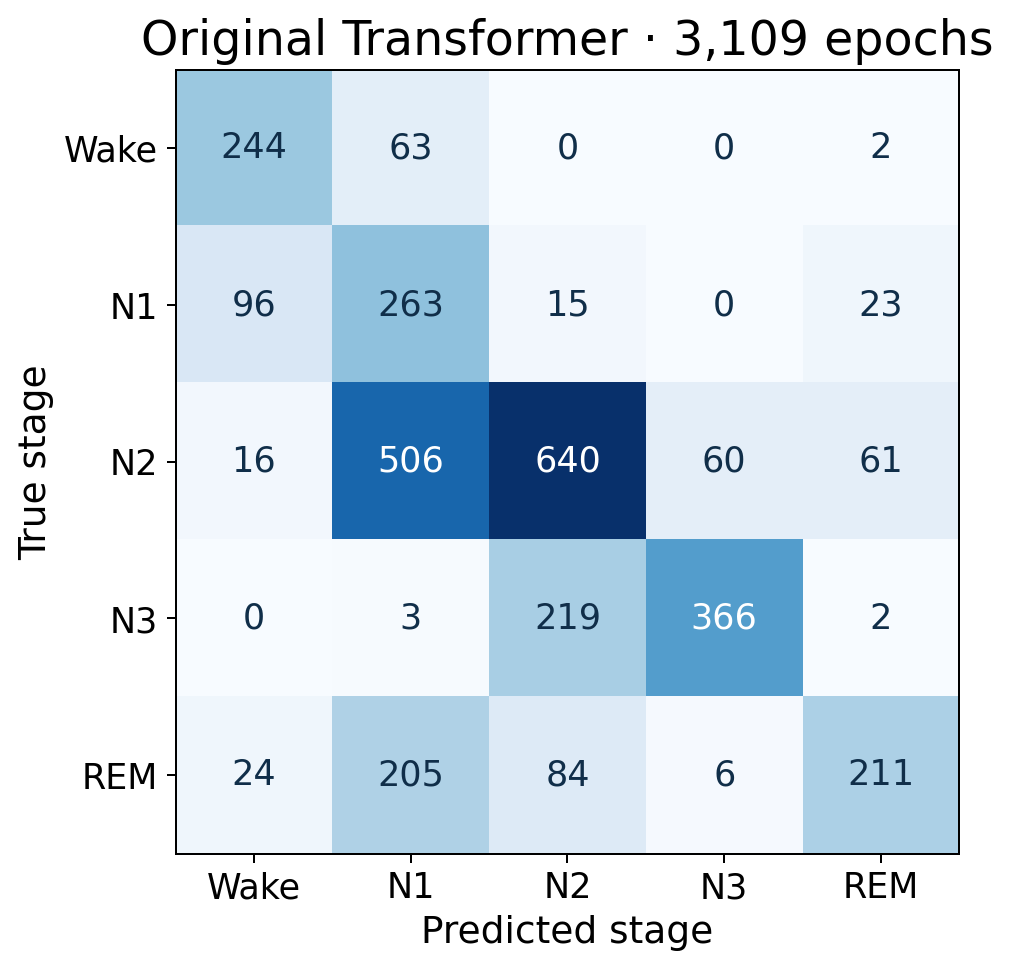
\includegraphics[width=130mm]{raw_confusion_matrix.png}
\caption{Retained classifier confusion matrix from the verified experiment. Rows are true stages and columns predicted stages.}\label{fig:raw-cm}
\end{figure}
\begin{figure}[htbp]
\centering
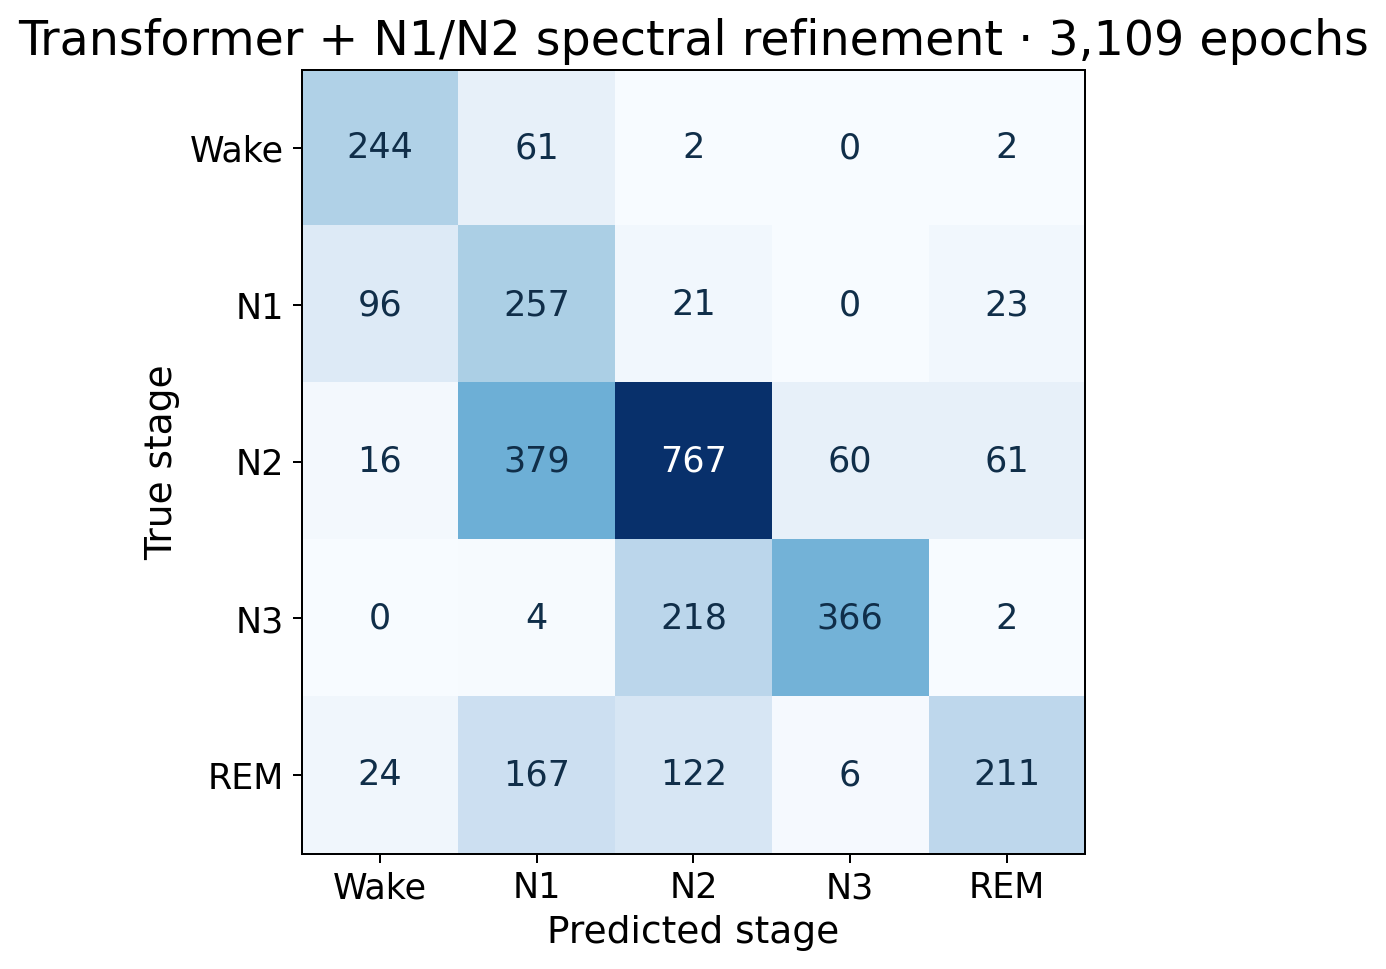
\includegraphics[width=130mm]{refined_confusion_matrix.png}
\caption{Confusion matrix after prediction-routed spectral refinement, on the same test epochs as Fig.~\ref{fig:raw-cm}.}\label{fig:refined-cm}
\end{figure}

\subsection{Hypnogram review and profiles}
Figure~\ref{fig:hypnogram} shows the retained SN009 hypnogram artifact. It supports inspection of stage sequences and localized disagreements, rather than independently establishing physiological cycle detection. Recording measurements and profiles can be exported alongside labels for review. SN001 must retain its 95-minute coverage qualification in any report; interpreting its reference deviation as a whole-night abnormality would be unsupported.

\begin{figure}[htbp]
\centering
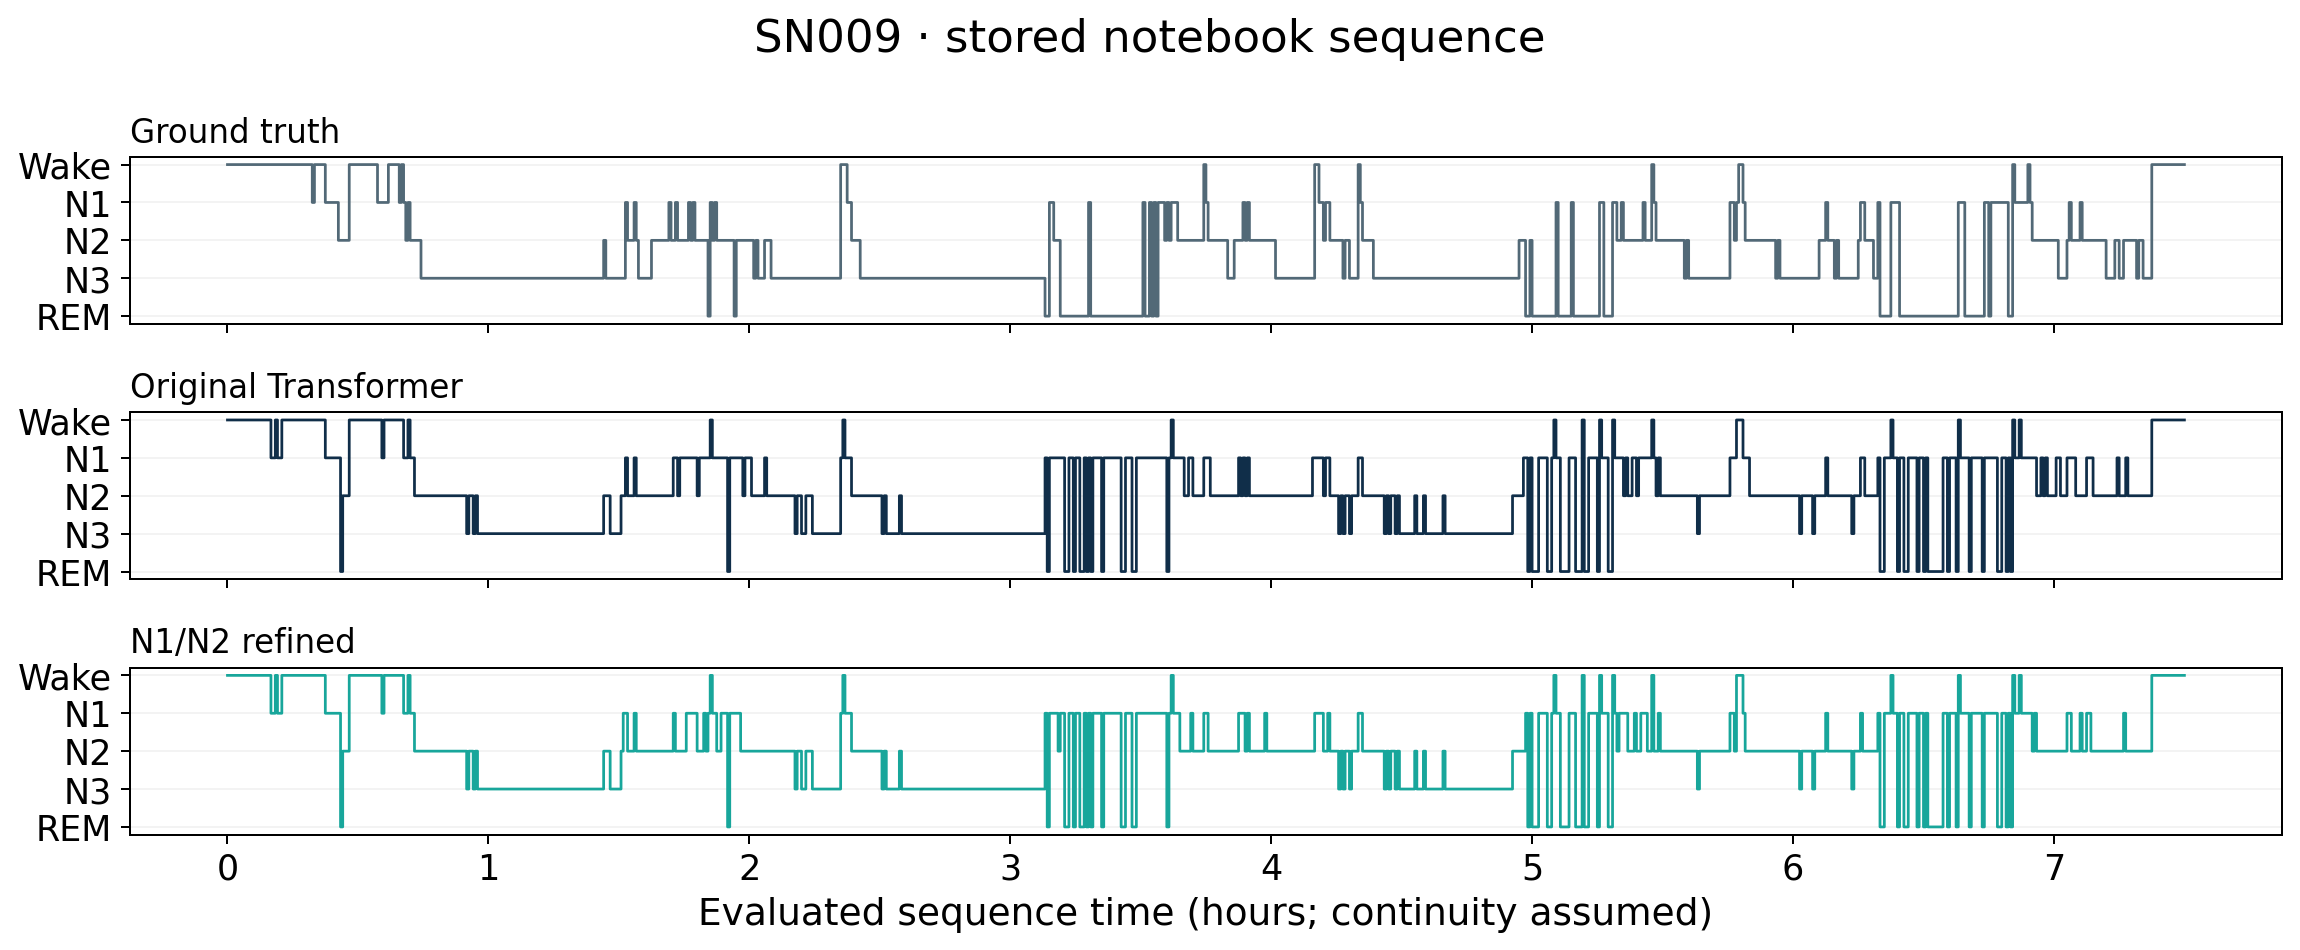
\includegraphics[width=\textwidth]{hypnogram_SN009.png}
\caption{Existing verified SN009 hypnogram comparing ground truth, the retained classifier, and N1/N2 refinement over the stored sequence. Epoch-index timing assumes continuity.}\label{fig:hypnogram}
\end{figure}

\section{Software implementation and reproducibility}\label{sec:software}
Sleep Studio provides the review interface for the pipeline. Its Windows client uses Electron and React, while a Python worker performs inference and measurement calculations. Users can inspect the saved experiment offline or run inference through the configured Ubuntu WSL--Colab connection. Checkpoint and signal inputs for live runs reside on mounted Drive storage. Results include hypnograms, baseline and refined scores, the original uncertainty values, and reference comparisons, with PDF, JSON, CSV, and ZIP exports. Imported inputs must satisfy the pipeline's channel, preprocessing, and timing requirements.

The main notebook is \path{Biomarker_N1_N2_Refinement.ipynb}. The reproduction script, \path{refinement_artifacts/reproduce.py}, loads the checkpoint and NPZs, extracts features, fits the training-only refiner, evaluates predictions, and builds reference statistics under \path{/content/eeg_refinement_audit}. The full checkpoint and signal arrays are supplied separately through Drive.

The authoritative current evidence resides in \path{refinement_artifacts/verified/}. It includes split metadata, per-epoch labels and predictions, classification reports, confusion matrices, fitted coefficients, reference tables, and plots. The recorded evaluation environment uses NumPy 2.1.3, TensorFlow 2.21.0, Keras 3.13.2, SciPy 1.16.3, and scikit-learn 1.6.1. The retained audit reports independent reproduction of saved metrics, coefficients, training counts, and profiles. Preparing this manuscript reuses those artifacts and does not constitute a fresh training or clinical validation run.

\section{Discussion and limitations}\label{sec:discussion}
The improvement is concentrated in the distinction the refiner was designed to revisit. Nevertheless, N1 F1 of 40.63\% and overall accuracy of 59.34\% show that many disagreements remain unresolved. Routing also places a firm limit on what can improve: an epoch assigned Wake, N3, or REM by the baseline never reaches the spectral decision. The reported gains therefore apply to this checkpoint and its matching feature pipeline.

Four test recordings provide limited evidence about performance on new patients, and successive epochs within a recording are correlated. We have not estimated confidence intervals or tested recording-level significance. There is also no evaluation on a locked external cohort or against clinical outcomes. The reference has a separate limitation: its architecture statistics come from predictions on the same small clinical training set used to construct the system. Gaps or incomplete coverage can further affect timing and comparisons. Validation of recording measurements and any claim about reviewer time savings would require additional studies.

Further limitations include absent explicit spindle detection, no dedicated formal slow-wave activity or spectral-edge-frequency metric, and no validated disease prediction. Baseline evidential uncertainty remains attached to the original five-class outputs. It should not be presented as calibrated confidence for the refined labels.

\section{Planned extensions}\label{sec:future}
The repository proposes a coarse Wake/REM/NREM classifier with an NREM expert for N1/N2/N3, potentially followed by a temporal CNN operating across consecutive epochs and probability calibration. These extensions are not implemented or evaluated in the current experiment. Future work should begin with EDF-to-epoch alignment and signal-quality audits, then use out-of-fold expert training, controlled ablations, a newly locked test cohort, and external dataset evaluation. Relevant outcomes include macro and class F1, calibration, inference latency, and errors in derived sleep measurements.

\section{Conclusion}
The workflow connects four-channel EEG staging, targeted spectral refinement, and descriptive profiles. Verified artifacts show 121 net additional correct test epochs without retraining the retained classifier. Recording coverage, cohort size, timing assumptions, and clinical interpretation limit these findings.

\section*{Acknowledgements}
We acknowledge project mentor Dr. Santosh Sathpathy. Authorship and contributions remain subject to team review.

\section*{Declarations}
\textbf{Manuscript status.} Initial project documentation draft. Target journal, corresponding author, contact details, author contributions, funding, and competing-interest statements require author confirmation before submission.

\textbf{Ethics.} The work uses the published HMC database. Any institution-specific secondary-use ethics determination has not been supplied and must be confirmed before submission; no approval or exemption is asserted here.

\textbf{Data availability.} HMC version 1.1 is available through PhysioNet~\cite{hmc2022}. The exact project split and derived experiment evidence are retained in the repository. Raw signals and the full checkpoint are external inputs.

\textbf{Code availability.} The current project notebook, reproduction scripts, desktop application, and verified artifacts are included in this codebase. A public archival repository URL or release DOI has not yet been specified.

\clearpage
\bibliography{references}
\end{document}
